\documentclass[tikz,border=6pt]{standalone}
\usepackage{pgfplots}
\pgfplotsset{compat=1.18}
\usepgfplotslibrary{colormaps}
\usetikzlibrary{arrows, arrows.meta, calc}
\usetikzlibrary{decorations.markings}


\usepackage{amssymb,amsmath,mathtools}

\usepackage[T1]{fontenc}
\usepackage[utf8]{inputenc}
\usepackage{newpxtext,newpxmath}
\usepackage{sectsty}

\renewcommand{\Re}{\operatorname{\mathrm{Re}}}
\renewcommand{\Im}{\operatorname{\mathrm{Im}}}

\begin{document}
	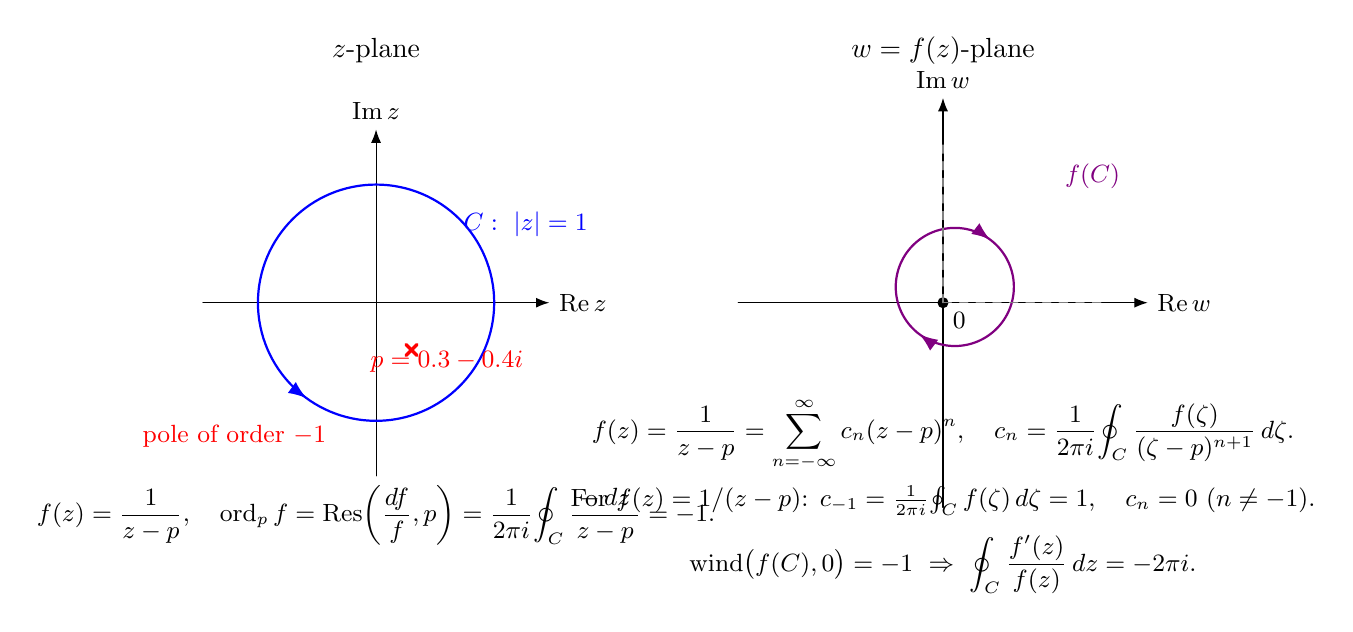
\begin{tikzpicture}[>=Latex, line cap=round, line join=round, font=\small]
		
		%========================
		% Left: z-plane
		%========================
		\begin{scope}[shift={(0,0)}]
			\node[font=\normalsize] at (0,3.2) {$z$-plane};
			% axes
			\draw[->] (-2.2,0)--(2.2,0) node[right] {$\Re z$};
			\draw[->] (0,-2.2)--(0,2.2) node[above] {$\Im z$};
			
			% unit circle C (positively oriented) -- radius 1.5 for visibility
			\draw[blue,thick,postaction={decorate},
			decoration={markings, mark=at position 0.65 with {\arrow{>}}}]
			(0,0) circle (1.5);
			\node[blue] at (1.9,1.0) {$C:\ |z|=1$};
			
			% pole at p (order -1), choose concrete p inside C
			\draw[red,very thick] (0.45,-0.6) ++(-0.07,-0.07) -- ++(0.14,0.14);
			\draw[red,very thick] (0.45,-0.6) ++(-0.07,0.07)  -- ++(0.14,-0.14);
			\node[red] at (0.9,-0.75) {$p=0.3-0.4i$};
			\node[red] at (-1.8,-1.7) {pole of order $-1$};
			
			% function label + order via winding form / logarithmic derivative
			\node[align=left] at (0,-2.7) {$\displaystyle
				f(z)=\frac{1}{z-p},\quad
				\operatorname{ord}_{p} f
				=\operatorname{Res}\!\left(\frac{df}{f},p\right)
				=\frac{1}{2\pi i}\!\oint_C \frac{-\,dz}{\,z-p\,}=-1.$};
		\end{scope}
		
		%========================
		% Right: w-plane = f(z)-plane
		%========================
		\begin{scope}[shift={(7.2,0)}]
			\node[font=\normalsize] at (0,3.2) {$w=f(z)$-plane};
			% axes
			\draw[->] (-2.6,0)--(2.6,0) node[right] {$\Re w$};
			\draw[->] (0,-2.6)--(0,2.6) node[above] {$\Im w$};
			
			% origin
			\fill (0,0) circle(2pt) node[below right] {$0$};
			
			% image curve f(C): z = 1.5 e^{it} -> w = 1/(z-p)
			% Let x = 1.5 cos t - 0.3, y = 1.5 sin t + 0.4  (so z-p = x + i y).
			% Then w = 1/(x+iy) = (x - i y)/(x^2 + y^2).
			\draw[violet,thick,
			postaction={decorate},
			decoration={markings,
				mark=at position 0.25 with {\arrow{>}},
				mark=at position 0.75 with {\arrow{>}}}]
			plot[domain=0:6.283, samples=650]
			({
				(1.5*cos(\x r) - 0.3) /
				( (1.5*cos(\x r) - 0.3)^2 + (1.5*sin(\x r) + 0.4)^2 )
			},
			{
				-(1.5*sin(\x r) + 0.4) /
				( (1.5*cos(\x r) - 0.3)^2 + (1.5*sin(\x r) + 0.4)^2 )
			});
			\node[violet] at (1.9,1.6) {$f(C)$};
			
			% dashed rays to visualize winding (clockwise once)
			\draw[gray,dashed] (0,0) -- (2.1,0);
			\draw[gray,dashed] (0,0) -- (0,2.1);
			
			% annotation: Laurent coefficient (residue) via Cauchy integrals around p
			\node[align=center] at (0,-2.45)
			{$\displaystyle
				f(z)=\frac{1}{z-p}=\sum_{n=-\infty}^{\infty} c_n (z-p)^n,\quad
				c_n=\frac{1}{2\pi i}\!\oint_C \frac{f(\zeta)}{(\zeta-p)^{n+1}}\,d\zeta.$\\[4pt]
				For $f(z)=1/(z-p)$: $c_{-1}=\frac{1}{2\pi i}\!\oint_C f(\zeta)\,d\zeta=1,\quad
				c_n=0\ (n\neq -1).$\\[6pt]
				$\mathrm{wind}\big(f(C),0\big)=-1
				\ \Rightarrow\
				\displaystyle \oint_C \frac{f'(z)}{f(z)}\,dz=-2\pi i.$};
		\end{scope}
		
	\end{tikzpicture}
\end{document}